
% \iffalse
\let\negmedspace\undefined
\let\negthickspace\undefined
\documentclass[journal,12pt,twocolumn]{IEEEtran}
\usepackage{cite}
\usepackage{amsmath,amssymb,amsfonts,amsthm}
\usepackage{algorithmic}
\usepackage{graphicx}
\usepackage{textcomp}
\usepackage{xcolor}
\usepackage{txfonts}
\usepackage{listings}
\usepackage{enumitem}
\usepackage{mathtools}
\usepackage{gensymb}
\usepackage{comment}
\usepackage[breaklinks=true]{hyperref}
\usepackage{tkz-euclide} 
\usepackage{listings}
\usepackage{gvv}                                        
\def\inputGnumericTable{}                                
\usepackage[latin1]{inputenc}                            
\usepackage{color}                                       
\usepackage{array}                                       
\usepackage{longtable}                                   
\usepackage{calc}                                        
\usepackage{multirow}                                    
\usepackage{hhline}                                      
\usepackage{ifthen}                                      
\usepackage{lscape}
\usepackage{amsmath}
\newtheorem{theorem}{Theorem}[section]
\newtheorem{problem}{Problem}
\newtheorem{proposition}{Proposition}[section]
\newtheorem{lemma}{Lemma}[section]
\newtheorem{corollary}[theorem]{Corollary}
\newtheorem{example}{Example}[section]
\newtheorem{definition}[problem]{Definition}
\newcommand{\BEQA}{\begin{eqnarray}}
\newcommand{\EEQA}{\end{eqnarray}}
\newcommand{\define}{\stackrel{\triangle}{=}}
\theoremstyle{remark}
\newtheorem{rem}{Remark}



\usepackage{amsmath} % Include the amsmath package for align environment

\begin{document}

\bibliographystyle{IEEEtran}

\vspace{3cm}

\title{NCERT Physics Chapter-15 Q7}
\author{EE23BTECH11059 - Tejas$^{}$}
\maketitle

\newpage

\Huge \textbf{QUESTION 7:} \\

\medskip
\Large
A hospital uses an ultrasonic scanner to locate tumors in a tissue. What is the
wavelength of sound in the tissue in which the speed of sound is $1.7 \, \text{km/s}$? The operating frequency of the scanner is $4.2 \, \text{MHz}$.

\bigskip
\Large
\textbf{SOLUTION:} \\
\begin{table}[h]
    \centering
    
    \begin{tabular}{|c|c|c|}
        \hline
        Input Parameter & Value & Description \\
        \hline
        $c$ & $1.7\times10^3$ & Speed of Wave  \\
        \hline
        $f$ & $4.2\times10^6$ & Frequency \\
        \hline
        
    \end{tabular}
    
\end{table} \\ \\
Wave equation for sound is: \\
$\begin{array}{ll}
\hspace{0.5cm} s(t)=s_{\text {max }}\cos(2\pi f t+\phi) \\ \\
\hspace{0.5cm}c=\frac{\Delta d}{\Delta t} ; \quad \Delta t=T \text { (Time period) } ,d=\lambda \text { (Wavelength) }  \\ 
\hspace{0.5cm}c=\frac{\lambda}{T}  \quad  \\ 
\hspace{0.5cm}c=f\lambda ; \quad \frac{1}{T}= f
\end{array}$ 



$\begin{array}{ll}
c= f \lambda \notag \\
\lambda = \frac{c}{f} \notag 
%\lambda &= \frac{1.7 \times 10^3}{4.2 \times 10^6} \, \text{m} \notag \\
%\lambda &= 4.047 \times 10^{-4} \, \text{m}
\end{array}$
\\
\\ \\ \\ \\ \\ \\

%Hence we substitute the input \\ parameters to get the answer \\ \\ \\ \\ \\ \\ \\ \\ \\ \\ \\ \\ \\ \\ \\ \\ \\ \\ \\ \\ 
Plotting the Sound Wave:
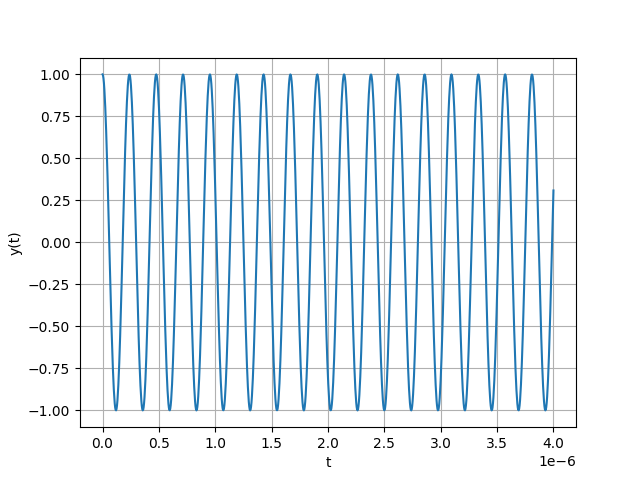
\includegraphics[scale=0.7]{images/plot.png}




        
        
        
             
             
        

        













\renewcommand{\thefigure}{\theenumi}
\renewcommand{\thetable}{\theenumi}





\end{document}
